\documentclass[a4paper,11pt]{article}
\usepackage[margin=25mm]{geometry}
\usepackage[T1]{fontenc}
\usepackage{lmodern}
\usepackage{amsmath,amssymb,amsthm,graphicx,booktabs,float}
\usepackage[hidelinks]{hyperref}
\setlength{\emergencystretch}{3em}
\newtheorem{theorem}{Theorem}[section]
\newtheorem{lemma}[theorem]{Lemma}
\newtheorem{proposition}[theorem]{Proposition}
\newtheorem{corollary}[theorem]{Corollary}
\hypersetup{pdftitle={Certified Frank-Wolfe stopping with a nonzero gradient at the minimum},pdfauthor={Yaroslav P. Lyakhov and Stepan A. Suvorov}}
\title{Certified Frank-Wolfe stopping\\with a nonzero gradient at the minimum}
\author{Yaroslav P. Lyakhov \and Stepan A. Suvorov}
\date{12 November 2026}
\begin{document}
\maketitle
\begin{abstract}
At a constrained minimum, the gradient can remain arbitrarily large.
We study stopping and step selection under gradient-dependent
smoothness for convex objectives on compact convex sets. A full-gap
certificate and quadratic backtracking give finite termination without
knowing the minimum value or requiring the gradient norm to vanish.
We count gradient and linear-oracle queries, rejected objective trials,
and adaptive directional-accuracy refinements. For product domains,
adding a normal linear term leaves the entire backtracking execution
unchanged when the method starts on the corresponding face. On the
globally $(1,1)$-smooth family $e^x+Ay$, a fixed gradient-norm step requires
at least a constant times $A$ updates, whereas backtracking is independent
of $A$. A deterministic experiment reproduces this separation with the
same stopping certificate for both methods.
\end{abstract}
\section{Introduction}
\label{sec:intro}
We consider minimization of a convex function over a compact convex set
$Q$. The function is twice continuously differentiable near $Q$ and
satisfies the gradient-dependent smoothness condition
\[
 \|\nabla^2 f(x)\|\le L_0+L_1\|\nabla f(x)\|,\qquad x\in Q.
\]
The constants $L_0,L_1$ and the diameter of $Q$ enter the work bounds;
the backtracking method does not require their values.
The smoothness condition and the algorithm do not use the unknown
minimum value. The point $x^*$ denotes a minimizer only in the analysis.

The full Frank-Wolfe gap
$G(x)=\max_{s\in Q}\langle\nabla f(x),x-s\rangle$
satisfies $f(x)-f(x^*)\le G(x)$ by convexity \cite{jaggi}.
Thus $f(x)-G(x)$ is a computable lower bound on the minimum.
This certificate remains valid at boundary solutions, where the
norm of the gradient may stay positive. The stopping quantity is the
gap, not the gradient norm.

Gradient-dependent smoothness nevertheless affects step selection.
We isolate this effect on the convex family
\[
 f_A(x,y)=\exp(x)+Ay,\qquad
 Q=[-1,1]\times[0,1],\qquad A>0.
\]
All members satisfy the same smoothness bound with $L_0=L_1=1$.
Starting at $(0.7,0)$, the full linear oracle always returns $(-1,0)$.
The gap and all objective values along the generated face are independent
of $A$, while the gradient norm grows with $A$.
We prove that the prescribed step in Algorithm~1 of Vyguzov and
Stonyakin \cite{vyguzov}, with fixed smoothness parameters, needs
$\Omega(A)$ updates even to cross $x=0$.
For exact oracle answers and the same initial curvature estimate,
quadratic backtracking gives identical trial points, accepted updates,
and stopping counts for every $A$.
This comparison concerns their fixed-parameter Algorithm~1; it does not
compare with their adaptive Algorithm~2.

We then give a stopping rule with adaptive absolute accuracy for the
directional oracle. Its error bounds certify both the full gap and the
descent direction. The rule carries the requested accuracy between
iterations, refines it when necessary, and retains the best certified
lower bound on the minimum. We prove termination at a prescribed
objective accuracy and bound all oracle calls and objective evaluations,
including failed precision checks, rejected backtracking trials, and the
final stopping query. Exact gradients and exact full linear minimization
are included as a special case.

\paragraph{Relation to earlier work.}
Gap certificates and approximate linear oracles are established parts
of convex Frank-Wolfe analysis \cite{jaggi}. Vyguzov and Stonyakin
\cite{vyguzov} study both fixed and adaptive steps under the smoothness
condition above. Quadratic backtracking also has an established analysis
\cite{pedregosa}; we use that update and provide the stopping rule and
complete query counts described here. The explicit family quantifies
how a gradient component can affect a norm-based step while leaving
the selected direction and its objective values unchanged.

The residual-dependent curvature condition used in warm-up analysis
\cite{warmup} is a different assumption and is not imposed here.
Local LMO \cite{locallmo} uses linear minimization over
$Q\cap B(x,t)$, whereas our rule retains the full linear oracle over $Q$.
The results therefore concern the original convex oracle model, with
no fixed-center regularity assumption or knowledge of $f(x^*)$.

\section{Model and computable information}
\label{sec:model}
Let $Q\subset\mathbb R^d$ be a nonempty compact convex set with
$\operatorname{diam}Q\le D$, where $D>0$. Let $f$ be convex on $Q$
and twice continuously differentiable on a neighborhood of $Q$. Assume
\begin{equation}\label{eq:gradient_smoothness}
 \|\nabla^2f(x)\|\le L_0+L_1\|\nabla f(x)\|,\qquad x\in Q,
 \quad L_0,L_1\ge0.
\end{equation}
Vector norms are Euclidean and matrix norms are spectral. A minimizer
$x^*\in Q$ exists. It is used to state the accuracy guarantee, not as an
input to the method. We write $f(x)-f(x^*)$ and $\|\nabla f(x)\|$
explicitly, without introducing names for these two expressions.

The available operations are objective evaluation, gradient evaluation,
and linear minimization over all of $Q$. The latter returns
\[
 s\in\arg\min_{v\in Q}\langle\nabla f(x),v\rangle.
\]
The full Frank-Wolfe gap is the computed quantity
\begin{equation}\label{eq:gap}
 G(x)=\max_{v\in Q}\langle\nabla f(x),x-v\rangle
     =\langle\nabla f(x),x-s\rangle.
\end{equation}
Since $x\in Q$, $G(x)\ge0$. Convexity gives
$f(x)-f(x^*)\le G(x)$, so $f(x)-G(x)$ is a valid lower bound on the
unknown minimum value \cite{jaggi}. In particular, the stopping test
does not evaluate that minimum.

At a constrained minimizer the correct first-order condition is
\[
 \langle\nabla f(x^*),v-x^*\rangle\ge0\quad(v\in Q),
\]
which is equivalent to $G(x^*)=0$. It does not require
$\nabla f(x^*)=0$. For example, $f(x)=Ax+x^2/2$ on $[0,1]$, $A>0$,
has its minimum at zero, derivative $A$ there, and Hessian equal to one.
A large gradient and large curvature are therefore different phenomena.

\begin{lemma}[A finite curvature bound from the initial gradient]
\label{lem:global_curvature}
The smoothness condition implies
\begin{equation}\label{eq:global_curvature}
 \|\nabla^2f(z)\|\le K_Q\quad(z\in Q),\qquad
 K_Q=(L_0+L_1\|\nabla f(x_0)\|)e^{L_1D}.
\end{equation}
Any sharper valid uniform bound can replace $K_Q$ in the results below.
This constant is used to express work bounds; the algorithm does not
need to know it.
\end{lemma}
\begin{proof}
For a unit direction $e$ along a segment from $x_0$ in $Q$, the
fundamental theorem of calculus gives
\[
 \|\nabla f(x_0+te)\|\le\|\nabla f(x_0)\|
 +\int_0^t\{L_0+L_1\|\nabla f(x_0+se)\|\}\,ds.
\]
For $L_1>0$, Gronwall's inequality bounds
$L_0+L_1\|\nabla f(x_0+te)\|$ by
$(L_0+L_1\|\nabla f(x_0)\|)e^{L_1t}$. Since $t\le D$, this proves
the assertion. If $L_1=0$, the original condition directly gives the
bound $L_0$.
\end{proof}

The smoothness condition contains no minimum value. The algorithm below
also uses neither a regularity constant centered at an unknown optimizer
nor a positive-distance assumption on that optimizer. Convexity is the
property that makes the full gap a global error certificate.

\section{Certified stopping with backtracking}
\label{sec:stopping}
Assume the convex model of Section~\ref{sec:model}. Convexity gives
\begin{equation}\label{eq:gap_certificate}
 f(x)-f(x^*)\le
 \langle\nabla f(x),x-x^*\rangle\le G(x).
\end{equation}
Thus the full gap is a computable error certificate even when
$\nabla f(x^*)\ne0$. No estimate of that unknown gradient is needed.
Use a positive global curvature bound $K_Q$ from
\eqref{eq:global_curvature} in the analysis; if that bound is zero,
it may be enlarged to any positive value. The algorithm does not
need $K_Q$, $L_0$, or $L_1$ as inputs.

\paragraph{Exact-oracle algorithm.}
Fix $\varepsilon>0$ and an initial stored curvature $L_{\rm init}>0$.
At a visited point $x$, compute its gradient, a full linear minimizer
$s\in Q$, and $G(x)$. Retain
\[
 \ell\leftarrow\max\{\ell,f(x)-G(x)\},
\]
where the first query initializes $\ell=f(x_0)-G(x_0)$.
Stop if $f(x)-\ell\le\varepsilon$. Otherwise set $d=s-x$, start with
half the previous accepted curvature (initially $L_{\rm init}$),
and double $L$ until
\begin{equation}\label{eq:stopping_bt}
 \alpha=\min\left\{1,\frac{G(x)}{L\|d\|^2}\right\},\qquad
 f(x+\alpha d)\le f(x)-\alpha G(x)+\frac{L\alpha^2\|d\|^2}{2}.
\end{equation}
Accept $x+\alpha d$, cache its objective value, and store $L$.
The update is ordinary Frank-Wolfe backtracking \cite{pedregosa}.
Objective values, gradients, and full linear minimizers are exact.

\begin{theorem}[Finite stopping and complete oracle counts]
\label{thm:finite_stopping}
Every line search terminates. The algorithm stops with
$f(x_N)-f(x^*)\le f(x_N)-\ell_N\le\varepsilon$.
If $G(x_0)>\varepsilon$, set
\[
 J=\left\lceil\log_2\frac{G(x_0)}{\varepsilon}\right\rceil,
 \quad b_j=G(x_0)/2^j\ (0\le j<J),
\]
\[
 H_{\rm init}=\left\lceil
 \log_2\max\left\{1,\frac{L_{\rm init}}{2K_Q}\right\}\right\rceil.
\]
The number $N$ of accepted updates satisfies
\begin{align}
 N&\le H_{\rm init}+\left\lceil\sum_{j=0}^{J-1}
       \max\left\{4,\frac{16K_QD^2}{b_j}\right\}\right\rceil
       \label{eq:stopping_steps}\\
  &\le H_{\rm init}+\left\lceil4J+
       \frac{32K_QD^2}{\varepsilon}\right\rceil.
       \label{eq:stopping_simple}
\end{align}
There are exactly $N+1$ gradient evaluations and $N+1$ full linear
minimization calls, including the terminal query. The initial objective
value and all accepted and rejected line-search trials number at most
\begin{equation}\label{eq:stopping_values}
 N_f\le 1+2N+
 \left\lceil\log_2\max\left\{1,\frac{2K_Q}{L_{\rm init}}\right\}\right\rceil.
\end{equation}
If $G(x_0)\le\varepsilon$, there are no updates and exactly one call
of each oracle; the phase quantities are unnecessary.
\end{theorem}

\begin{proof}
Every retained $\ell$ is a lower bound on $f(x^*)$, so
\[
 0\le f(x)-f(x^*)\le f(x)-\ell\le G(x).
\]
A nonterminal point therefore has $G(x)>0$ and $d\ne0$.
Every $L\ge K_Q$ passes \eqref{eq:stopping_bt}. Accepted values obey
\begin{equation}\label{eq:stopping_progress}
 \begin{split}
 L_k&\le\max\{L_{k-1}/2,2K_Q\},\qquad L_{-1}=L_{\rm init},\\
 f(x_k)-f(x_{k+1})&\ge
 \min\left\{\frac{G(x_k)}2,\frac{G(x_k)^2}{2L_kD^2}\right\}.
 \end{split}
\end{equation}
Thus the objective decreases, $\ell$ increases, and $f(x_k)-\ell_k$
decreases. If $L_k>2K_Q$, the accepted trial was the first: otherwise
its preceding rejected value $L_k/2>K_Q$ would have passed.
Such an update halves the inherited curvature. Once $L_k\le2K_Q$,
it stays at most $2K_Q$. There are at most $H_{\rm init}$ updates
above this threshold.

Assign every other nonterminal update to
$b_j/2<f(x_k)-\ell_k\le b_j$. These phases are visited in order.
Here $G(x_k)>b_j/2$, and \eqref{eq:stopping_progress} gives decrease
at least
\[
 \min\left\{b_j/4,\ b_j^2/(16K_QD^2)\right\}.
\]
The total decrease of all updates starting in that phase is at most
the true error at its entry, hence at most $b_j$. This includes the
last update leaving the phase, because its endpoint has objective
at least $f(x^*)$. Division and summation prove
\eqref{eq:stopping_steps}. The inequality
$\sum_{j<J}b_j^{-1}<2/\varepsilon$ gives
\eqref{eq:stopping_simple}. The same finite bound applies to every
unfinished prefix, excluding an infinite nonterminal run.

If update $k$ rejects $q_k$ trials, then
$L_k=2^{q_k-1}L_{k-1}$. For $N\ge1$,
\[
 \sum_{k<N}(q_k+1)=2N+\log_2\frac{L_{N-1}}{L_{\rm init}},
 \quad L_{N-1}\le\max\{L_{\rm init}/2^N,2K_Q\}.
\]
Adding the initial objective value proves \eqref{eq:stopping_values}.
Each visited point uses one gradient and one full linear minimizer.
\end{proof}

\subsection{Carrying absolute directional accuracy between iterations}
A directional query with requested accuracy $\eta>0$ returns $h\ge0$
and $d=s-x$, $s\in Q$, with certified bounds
\begin{equation}\label{eq:directional_query}
 G(x)\le h+\eta,\qquad
 -\langle\nabla f(x),d\rangle\ge h-\eta.
\end{equation}
This is an explicit oracle requirement, not a consequence of the line-search
check. Objective values remain exact. The exact algorithm above needs
no such additional oracle.

Start with $\eta_0>0$ and fix $0<\theta<1$. After every query, update
$\ell\leftarrow\max\{\ell,f(x)-(h+\eta)\}$ and first test
$f(x)-\ell\le\varepsilon$. If this fails and $\eta>\theta h$,
halve $\eta$ and query again at the same point, reusing its objective
value. Once $\eta\le\theta h$, use \eqref{eq:stopping_bt} with
$G(x)$ replaced by $h-\eta$. Carry the current $\eta$ to the next point.

\begin{corollary}[All accuracy refinements are counted]
\label{cor:directional_stopping}
The rule stops with $f(x_N)-f(x^*)\le\varepsilon$.
Put $\kappa=(1-\theta)/(1+\theta)$. The total number $R$ of accuracy
halvings obeys
\begin{equation}\label{eq:accuracy_refinements}
 R\le\left\lceil\log_2\max\left\{1,
 \frac{(1+\theta)\eta_0}{\theta\varepsilon}\right\}\right\rceil.
\end{equation}
If the first upper gap $h_0+\eta_0>\varepsilon$, define $J$ and $b_j$
as above with $G(x_0)$ replaced by $h_0+\eta_0$. Then
\begin{equation}\label{eq:directional_steps}
 N\le H_{\rm init}+\left\lceil
 \frac{4J}{\kappa}+\frac{32K_QD^2}{\kappa^2\varepsilon}
 \right\rceil.
\end{equation}
There are exactly $N+1+R$ directional queries. The objective bound
\eqref{eq:stopping_values} is unchanged. If each directional query uses
one full linear minimization call, their number is also $N+1+R$.
If the first upper gap is at most $\varepsilon$, the rule stops immediately.
\end{corollary}
\begin{proof}
At a failed nonterminal accuracy check,
\[
 \varepsilon<f(x)-\ell\le h+\eta
 <(1+\theta)\eta/\theta.
\]
Since $\eta$ is halved and never reset, this proves
\eqref{eq:accuracy_refinements}. At a passed nonterminal check,
\[
 h-\eta\ge\kappa(h+\eta)\ge\kappa(f(x)-\ell)>0.
\]
The preceding descent and phase proof therefore applies with phase
slope threshold $\kappa b_j/2$, giving
\eqref{eq:directional_steps}. Each visited point has one closing query,
including the terminal point, and each halving adds one failed query.
Refinements at a fixed point do not evaluate the objective again.
\end{proof}

The stopping proof uses the full gap and permits a nonzero limiting
gradient. In Section~\ref{sec:normal}, the true curvature bound and the
complete execution are independent of an arbitrarily large normal
gradient. Directional-query counts specify how often the requested
accuracy is needed; the cost of producing each answer is determined by
the chosen oracle implementation.

\section{Large normal gradients and unchanged trajectories}
\label{sec:normal}
The gradient-dependent curvature bound can grow because of a linear
term that has no curvature. The next result identifies a family on
which this growth has no effect on the backtracking method.

\begin{proposition}[Invariance under a normal linear term]
\label{prop:normal_invariance}
Let $Q_0$ be compact and convex, and let $\varphi$ be convex and $C^2$
near $Q_0$. For $A\ge0$, consider
\[
 Q=Q_0\times[0,1],\qquad f_A(z,y)=\varphi(z)+Ay.
\]
Run the exact method of Section~\ref{sec:stopping} from $(z_0,0)$,
with the same accuracy and initial curvature. Choose the same
linear minimizer on $Q_0$ in every tie, and choose $y=0$ in ties.
Then all iterates, gaps, accepted step sizes, backtracking trials, and
oracle counts are identical for all $A\ge0$. If $\varphi$ satisfies
\eqref{eq:gradient_smoothness}, every $f_A$ satisfies it with the same
constants. At a minimizer $(z^*,0)$,
\[
 \|\nabla f_A(z^*,0)\|
   =\sqrt{\|\nabla\varphi(z^*)\|^2+A^2}\ge A.
\]
\end{proposition}
\begin{proof}
At $(z,0)$ the gradient is $(\nabla\varphi(z),A)$, so a full linear
minimizer is $(s,0)$ with $s$ minimizing
$\langle\nabla\varphi(z),s\rangle$ on $Q_0$. The direction has zero
last coordinate. Its norm, its directional derivative, the gap, and
every objective value along it are independent of $A$. The retained
lower bound and every backtracking comparison are consequently the
same. Induction proves the equality of the complete executions.
The Hessian has blocks $\nabla^2\varphi$ and zero, while
$\|\nabla f_A\|\ge\|\nabla\varphi\|$, proving the smoothness claim.
\end{proof}

A bound on $\|\nabla^2\varphi\|$ on $Q_0$ supplies a value of $K_Q$
independent of $A$ in Theorem~\ref{thm:finite_stopping}. Thus both the
actual execution and a valid work bound can ignore this normal
component. No inverse Hessian is used.

\subsection{A quantitative comparison with the fixed smoothness step}
The fixed-parameter rule in Algorithm~1 of \cite{vyguzov} uses
\begin{equation}\label{eq:vyguzov_step}
 \alpha_k=\min\left\{1,
 \frac{G(x_k)}{e(L_0+L_1\|\nabla f(x_k)\|)\|s_k-x_k\|^2}
 \right\}.
\end{equation}
Here $e$ is the base of the natural logarithm. We compare this specified
rule with backtracking; the adaptive Algorithm~2 in that work is a
different method.

\begin{theorem}[A linear separation in the normal coefficient]
\label{thm:normal_separation}
Let
\[
 f_A(x,y)=e^x+Ay,\qquad Q=[-1,1]\times[0,1],\qquad A>0.
\]
Start at $(a,0)$, where $0<a<1$, and require
$0<\varepsilon<1-e^{-1}$. Use $L_0=L_1=1$ in
\eqref{eq:vyguzov_step}, and stop by the same retained lower-bound
test as in Section~\ref{sec:stopping}. This rule needs at least
\begin{equation}\label{eq:normal_lower}
 \left\lceil a e^{1-a}A\right\rceil
\end{equation}
updates before it can stop. The backtracking execution, including its
finite stopping time, is independent of $A$.
\end{theorem}
\begin{proof}
The functions are globally convex, with
\[
 \nabla f_A(x,y)=(e^x,A),\qquad
 \nabla^2f_A(x,y)=\operatorname{diag}(e^x,0).
\]
Thus \eqref{eq:gradient_smoothness} holds globally with the fixed
constants $L_0=L_1=1$. The minimum on $Q$ is at $(-1,0)$.
Every full linear oracle returns $(-1,0)$. The iterates stay on $y=0$
and their first coordinates decrease. At a current coordinate $x$,
the gap is $e^x(x+1)$. Rule~\eqref{eq:vyguzov_step} decreases $x$ by
at most
\[
 \frac{e^x}{e(1+\sqrt{e^{2x}+A^2})}
 \le\frac{e^a}{eA}.
\]
This remains an upper bound when the step is capped at one. Until the
coordinate crosses zero, the true objective error is at least
$1-e^{-1}>\varepsilon$, so no valid certificate permits stopping.
Moving a distance at least $a$ proves \eqref{eq:normal_lower}.
Backtracking invariance follows from Proposition~\ref{prop:normal_invariance}.
Its finite stopping follows from Theorem~\ref{thm:finite_stopping},
for example with $K_Q=e$ and $D=\sqrt5$, both independent of $A$.
\end{proof}

The separation concerns a concrete convex family and a specified step
rule. Its cause is visible in \eqref{eq:vyguzov_step}: the normal
component enters the denominator even though it changes neither the
objective along the executed steps nor the Hessian. Backtracking tests
the actual change along those steps.

\section{A reproducible boundary experiment}
\label{sec:experiments}
We evaluate the family in Theorem~\ref{thm:normal_separation} with
$a=0.7$, $\varepsilon=10^{-6}$, $L_{\rm init}=1$, and
$A\in\{0,1,10,100,1000\}$. The comparison uses
\eqref{eq:vyguzov_step} with $L_0=L_1=1$ and the exact-oracle
backtracking rule. Both retain the same lower-bound certificate.
The full box linear oracle uses a fixed tie rule. There is no sampling
or parameter tuning across these ten deterministic runs.

\begin{table}[H]
\centering
\caption{Accepted updates and objective calls. Every backtracking run
uses three gradients and three full linear minimizations.}
\label{tab:boundary}
\begin{tabular}{rrrrr}
\toprule
$A$ & Fixed rule & Backtracking & Fixed $N_f$ & Backtracking $N_f$\\
\midrule
0    & 11   & 2 & 12   & 5\\
1    & 14   & 2 & 15   & 5\\
10   & 66   & 2 & 67   & 5\\
100  & 610  & 2 & 611  & 5\\
1000 & 6045 & 2 & 6046 & 5\\
\bottomrule
\end{tabular}
\end{table}

All runs stop at $(-1,0)$ with zero gap. The backtracking traces agree
exactly across the five values of $A$: the first accepted curvature is
two, the second is one, and there are two rejected trials in total.
At $A=1000$, the gradient norm at the solution is approximately
$1000.000068$, while the objective error and the certificate are zero.

\begin{figure}[H]
\centering
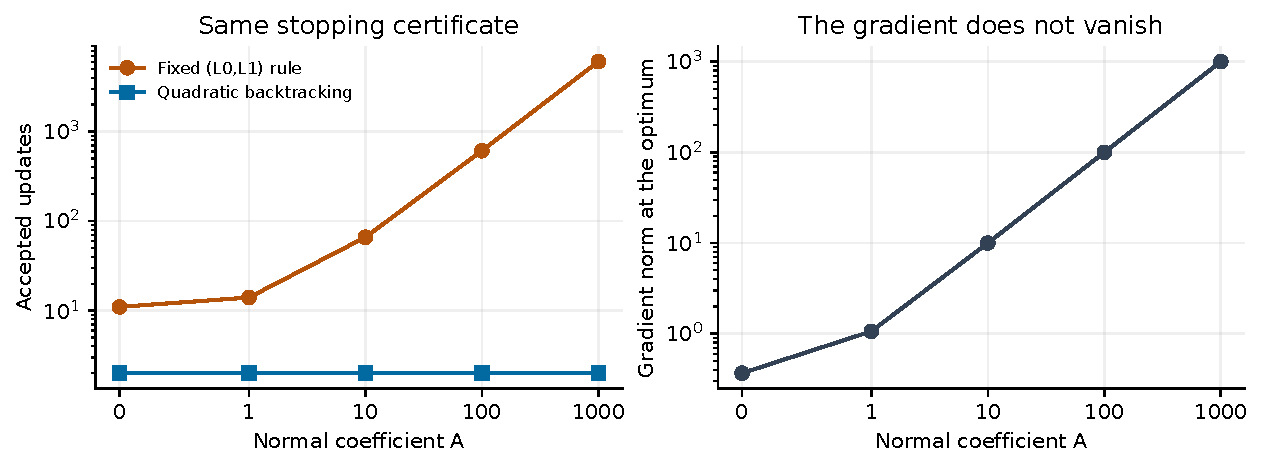
\includegraphics[width=\linewidth]{figures/boundary_normal_benchmark.pdf}
\caption{The fixed norm-based step becomes smaller as the normal
coefficient grows. Backtracking has the same two-update execution,
although the gradient at the minimizer grows without bound.}
\label{fig:boundary}
\end{figure}

The script \texttt{Code/benchmark\_boundary.py} writes every visited
point, gap, retained certificate, accepted curvature, and oracle count.
It checks feasibility, objective decrease, the analytical crossing
bound~\eqref{eq:normal_lower}, and equality of the backtracking traces.
The known solution is used only for a diagnostic after stopping.
The algorithm itself receives neither the minimizer nor its value.
The experiment uses Python floating-point arithmetic; the statements
in Sections~\ref{sec:stopping} and~\ref{sec:normal} are proved
independently of these numerical checks.

\paragraph{Reading the result.}
The full gap resolves the stopping issue at a boundary minimum.
Quadratic backtracking also avoids an unnecessary dependence on the
normal coefficient in the product family of
Proposition~\ref{prop:normal_invariance}. The comparison in
Table~\ref{tab:boundary} uses the fixed Algorithm~1 of~\cite{vyguzov};
the proof and the table make the same comparison.

\paragraph{Use of computational tools.}
AI tools assisted with derivations, checks, implementation, and writing.
The authors are responsible for validating the mathematical claims,
sources, and reported computations.

\begin{thebibliography}{99}
\bibitem{jaggi}M.~Jaggi.
Revisiting Frank-Wolfe: Projection-Free Sparse Convex Optimization.
\emph{Proceedings of the 30th International Conference on Machine Learning},
PMLR 28(1):427-435, 2013.
\url{https://proceedings.mlr.press/v28/jaggi13.html}.

\bibitem{vyguzov}A.~A.~Vyguzov and F.~S.~Stonyakin.
Frank-Wolfe Algorithms for $(L_0,L_1)$-smooth functions.
\href{https://arxiv.org/abs/2510.16468v5}{arXiv:2510.16468v5}, 2026.

\bibitem{pedregosa}F.~Pedregosa, G.~Negiar, A.~Askari, and M.~Jaggi.
Linearly Convergent Frank-Wolfe with Backtracking Line-Search.
\emph{Proceedings of the Twenty Third International Conference on
Artificial Intelligence and Statistics}, PMLR 108:1-10, 2020.
\url{https://proceedings.mlr.press/v108/pedregosa20a.html}.

\bibitem{warmup}F.~Alimisis, R.~Islamov, and A.~Lucchi.
Why Do We Need Warm-up? A Theoretical Perspective.
\href{https://arxiv.org/abs/2510.03164v2}{arXiv:2510.03164v2}, 2026.

\bibitem{locallmo}P.~Richt\'{a}rik, K.~Gruntkowska, and H.~Li.
Local LMO: Constrained Gradient Optimization via a Local Linear
Minimization Oracle.
\href{https://arxiv.org/abs/2605.08850v1}{arXiv:2605.08850v1}, 2026.
\end{thebibliography}

\end{document}
